\chapter{Design}
This chapter describes the design of the application to be built, this design is based on the requirements gathered previously. The design has to
incorporate solutions to the problems mentioned in section \hyperref[sec:problems]{Problems}.
This means the design has to include classes for a back-end using swift, a frontend using Samsung\textquotesingle s SDK, a sandbox workaround and a
 means for inter-TV communication. First we will discuss the current software archictecture on the TV. Then we will discuss an extended version of
 this architecture which will allow us to implement solutions for the aforementioned problems. Finally the class diagram and other UML models will be discussed.

\section{Standard Samsung Software Architecture}
As mentioned before in section \hyperref[sec:problems]{Problems}
the Samsung SDK for the SmartTV only allows programmers to create applications using HTML, CSS, Javascript and Flash.
All operations to be performed in the root file system will go via the SDK as a middle layer between our app and the root file system. This is
because the Samsung SDK provides a set of methods in which this can be realised.

\begin{center}
\begin{figure}[h]
	\centering
	\mbox{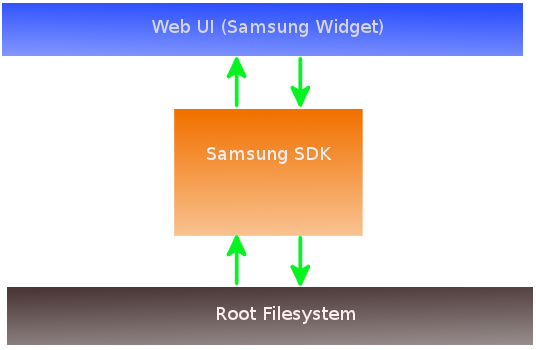
\includegraphics[width=1\textwidth]{Images/original_architecture.png}}
	\caption{The original architecture created by Samsung.}
	\label{fig:original_architecture}
\end{figure}
\end{center}

\clearpage

\section{Extended Software Architecture}
The solution for being able to run custom made code has already been mentioned, namely getting root access to the TV.
This was already done in the orientation phase of this project. This leaves only one problem, the sandbox.
The frontend and back-end of our application need a way to communicate. It is not possible to perform direct calls to the back-end, because the 
Samsung SDK is completely sandboxed. Therefore we decided to use a networking approach, so the frontend and back-end will act as seperate 
applications, communicating via a network (client-server architecture).

In the Samsung SDK it is possible to send HTTP GET messages to any server and since we already have root access, it is possible to implement
our own HTTP web server. This way one can create a bridge between the client software using Samsung\textquotesingle s framework and our own made 
HTTP Server. Since the TV does not support HTML5 we were not able to use websockets which provide an open connection in which a reply can be 
received asynchronously at any time. Thus, we are restricted to the client-server architecture where you have to keep polling to obtain an updated value for the progress of a download for example or an updated list of search results. 

The server is seperated in three subsystems. These are the HTTP server, which handles HTTP requests and acts as a controller, the Download Engine and the Search Engine, which makes use of dispersy and DHT implemented by the tribler team. This can also be seen in figure \ref{fig:architecture}.

\begin{center}
\begin{figure}[h]
	\centering
	\mbox{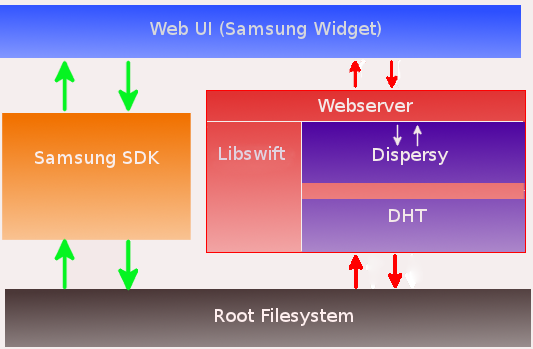
\includegraphics[width=1\textwidth]{Images/architecture.png}}
	\caption{The adjusted architecture with our application. Our application is injected as a webserver daemon, here seen in red. 
	The purple part is developed by the Tribler team, with which we have to communicate.}
	\label{fig:architecture}
\end{figure}
\end{center}
\clearpage

\section{Class Diagram}
Figure \ref{fig:class_server} shows the class diagram for the webserver. These classes are then explained in more detail.

\subsection{Download}
A data structure to store all information regarding downloads from the swift engine and as an interface to the swift methods.
This information can be accessed by the DownloadManager, which publishes the information of all Downloads to the web interface via
the HttpServer class. This information can be retrieved by using swift methods. Core functionality of this class is based on the swift engine.
In that sense, it is a wrapper class which makes use of swift methods.

\subsection{Stream}
This class serves as a data structure to store all information regarding streams from the swift engine and as interface to the swift methods. It 
is in essence the live-on-demand counterpart of the Download class, which is used to retrieve files from the Internet to store them on disk.
Since there will always be only one stream opened at a time (assuming that people only watch one film at the same time),
this class is designed according to the Singleton pattern.

\subsection{DownloadManager}
The DownloadManager, as the name implies, holds a list of Downloads and manages them. It can be accessed by the HttpServer, which controls this
class whenever needed. It retrieves information from all Downloads and calls the methods of the correct Download. The DownloadManager also manages
 the Stream class. In order to save bandwidth, all Downloads are paused when a stream is opened. This is why the Stream class is also managed by
 the DownloadManager, because that way the DownloadManager is able to access both the Stream class and the Download class. For similar reasons as
 the HttpServer class, the DownloadManager is designed to be a static class.

\subsection{SearchEngine}
This class serves as the interface to the search functionality developed by the Tribler team. It starts dispersy and DHT,
with which files can be sought on the net by calling the methods in the dispersy module. For similar reasons as the HttpServer class and
DownloadManager class, this class is designed to be a static class.

